\chapter{Simulação das Regras}
\label{chap:rules}

Nesta sessão serão abordados tópicos chave para a utilização das regras no sistema
IDS/IPS, que são responsáveis por definir quais tipos de tráfego, assinaturas e
pacotes serão interpretados e, porteriormente, barrados.

\section{Utilização das Regras}
Com a finalidade de deixar a cargo do usuário escolher quais tipos de ataque este deseja
que o sistema de detecção de intrusos trate, as aplicações Snort e Suricata permitem
que sejam editadas, adicionadas e removidas regras de captura de dados na rede.


Cada regra tem uma sequência de informações que pode ser editada pelo usuário.
Uma regra utilizada para capturar pacotes utilizando o serviço ping é exemplificada
a seguir:


\begin{framed}
alert tcp \$EXTERNAL NET any -> \$HOME NET 5900:5920 (msg:"ET SCAN
Potential VNC Scan 5900-5920"; flags:S,12; threshold: type both, track by src,
count 5, seconds 60; reference:url,doc.emergingthreats.net/2002911;
classtype:attempted-recon; sid:2002911; rev:5;)
\end{framed}

Esta regra possui um conjunto de comandos significativos para que esta funcione
corretamente:

\begin{itemize}
  \item o primeiro comando "alert", representa que o usuário deseja ser alertado quando
  essa regra for identificada;
  \item  "tcp", indica qual protocolo será utilizado para esta;
  \item "EXTERNAL NET", representa onde ela irá supervisionar o tráfego, neste caso é um
  conjunto de IP's configurado na variável local na rede 192.168.0.0/16;
  \item "ET SCANPotential VNC Scan 5900-5920", é a mensagem sinalizada ao usuário no momento
  em que for identificada;
  \item "reference:url,doc.emergingthreats.net/2002911;",
 representa o repositório das regras onde este vai buscar os padrões de pacotes
 com o código 2002911, que sinaliza o tráfego ICMP quando se utiliza o Ping.
\end{itemize}

O Snort e o Suricata fornecem repositórios com regras que são atualizados constantemente
de acordo com os novos ataques e vulnerabilidades que são encontrados recorrentemente nos
 sistemas. O repositório do Snort oferece um versionamento constante com os logs
 das novas regras adicionadas desde a última atualização disponível em \cite{snortRules}. O
 Suricata também oferece um serviço de atualização das regras, o Oinkmaster,
 além de uma aplicação web contento os novos updates caso o usuário opite por
 não usar o Oinkmaster em \cite{suricataRules}.

 \section{Manipulação de Regras}
 Para editar, adicionar e remover uma regra ou um conjunto de regras, alguns passos
 são necessários: Identificar Regra, Restringir Regra e Atualizar Conjunto de Regras,
 que serão descritos a seguir.

 \subsection{Identificação de Regra}
 Quando há um tráfego de dados que o sistema IDS/IPS julga como ruído a partir das
 regras definidas, este reporta no Snorby os detalhes desses pacotes. A seguir
 é ilustrado na figura \ref{fig:regra_ping_ativa} a ação de um atacante(192.168.0.16)
 utilizando a funcionalidade Ping com o ping da servidor Snort (192.168.0.42).

 \begin{figure}[h]
  \centering
  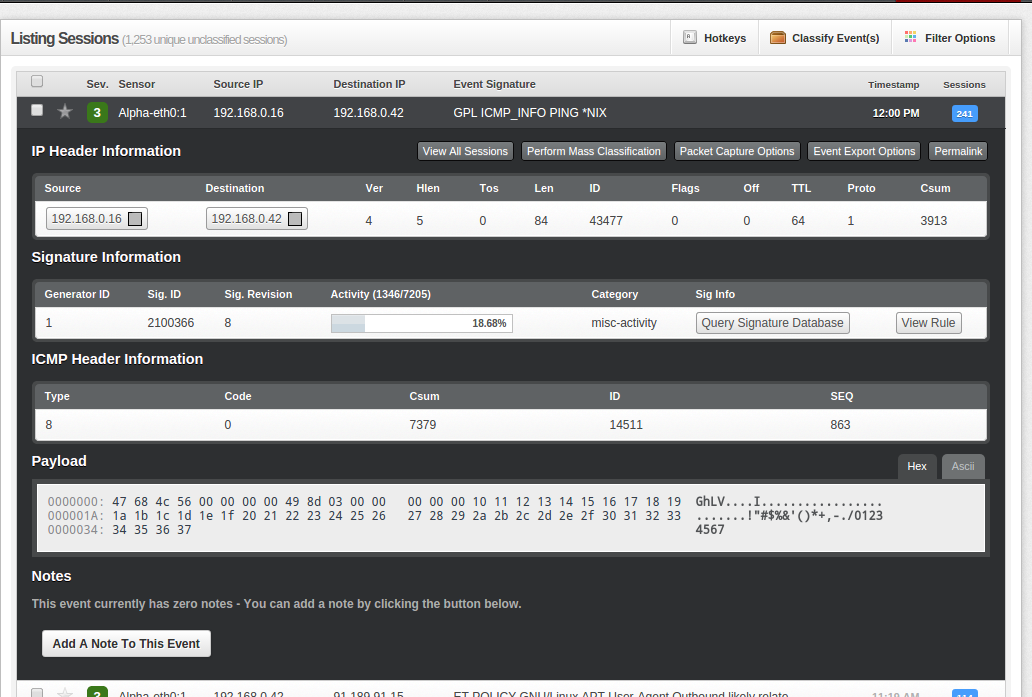
\includegraphics[width=400px, scale=1]{resource/regra_ping_ativa}
  \caption{Vítima - regra de ping ativa}
\label{fig:regra_ping_ativa}
\end{figure}

É possível identificar mensagem informada \"GPL ICMP INFO PING NIX\", bem como
o Genarator ID e Seg. ID da regra, respectivamente: 1 e 2100366. Esses dois
números são responsáveis por identificar uma regra de maneira particular.
Para este caso de demonstração, iremos desabilitar esta regra utilizando o Genarator
ID e o Seg. ID.

\subsection{Restrição de Regras}
A restrição de regras é feita no diretório de configuração dessas, quando utilizado
o modo padrão, localizado em /ect/nsm/pulledpork/disablesid.conf, representado a
seguir na figura \ref{fig:comando_desabilita_regra_ping}.

 \begin{figure}[h]
  \centering
  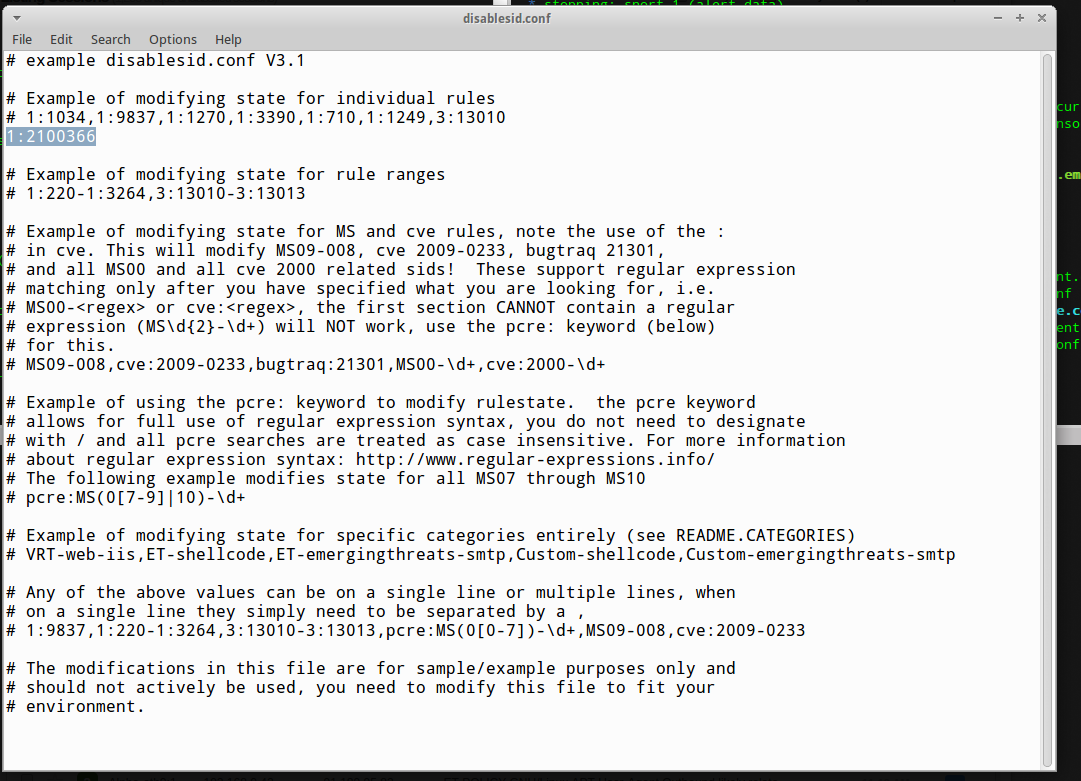
\includegraphics[width=400px, scale=1]{resource/comando_desabilita_regra_ping}
  \caption{Vítima - comando para desabilitar a regra do ping}
\label{fig:comando_desabilita_regra_ping}
\end{figure}

Para desabilitar, devem ser passados os identificadores citados acima, de maneira
que para desabilitar, devem ser passados os Genarators:Seg separados por vírgula
para cada regra. Neste exemplo, para desabilitar o Ping, foi passado 1:2100366.

\subsection{Atualização das Regras}
Sempre que o set de regras for editado, removido ou adicionado, deve-se atualizar
as aplicações que estão em funcionamento para que as alterações sejam aplicadas.
Como o Ping foi desabilitado, o comando rules-update deve ser utilizado, de acordo
com a figura \ref{fig:rule_update} a seguir. Este se
encontra no diretório /usr/bin/rules-update por padrão.

 \begin{figure}[h]
  \centering
  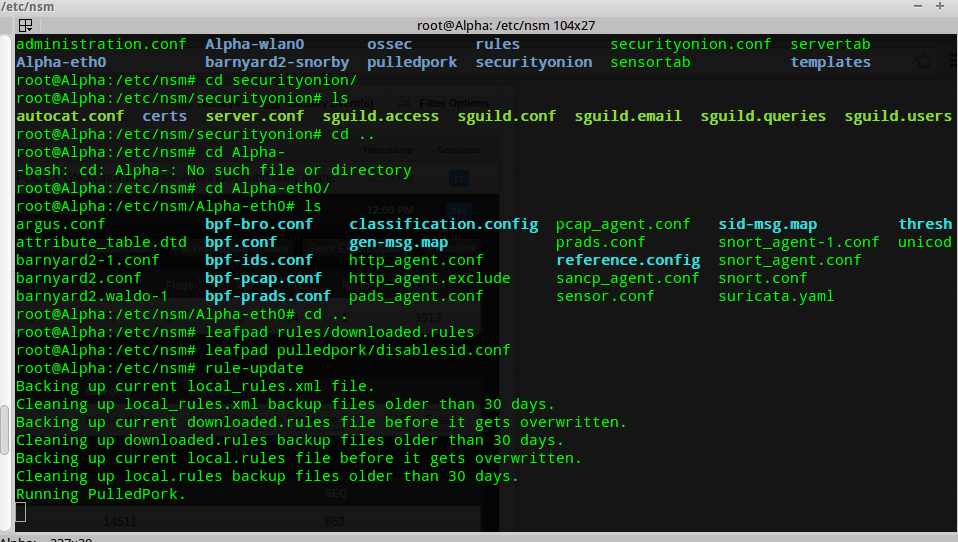
\includegraphics[width=400px, scale=1]{resource/rule_update}
  \caption{Vítima - Comando para atualizar as ferramentas para ignorar a regra do ping}
\label{fig:rule_update}
\end{figure}

Após utilizar este comando, é possível observar que a regra foi comentada no banco
que o sistema utiliza, conforme a figura \ref{fig:regra_desativada}.

 \begin{figure}[h]
  \centering
  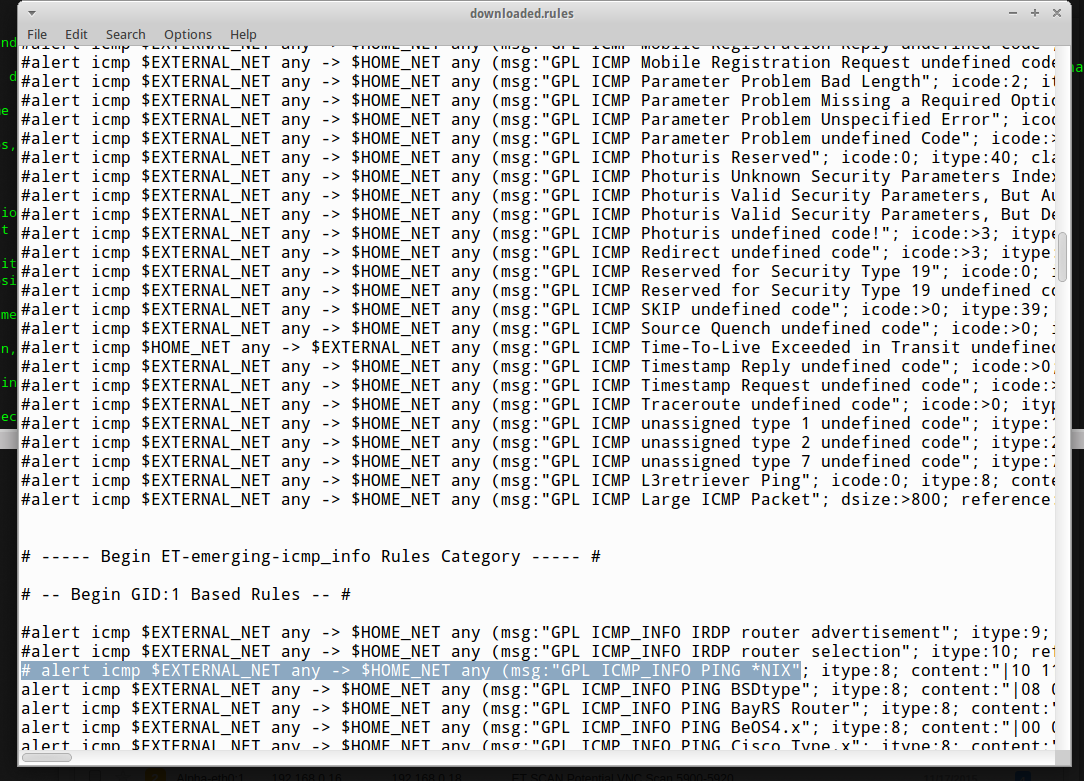
\includegraphics[width=400px, scale=1]{resource/regra_desativada}
  \caption{Vítima - regra de ping desabilitada}
\label{fig:regra_desativada}
\end{figure}

Dessa maneira, após a remoção da regra, uma nova solicitação do Ping foi feita
 pelo atacante, porém, o IDS/IPS não identificou o tráfego. Para reativar a regra,
 basta apenas apagar o restrição informada no arquivo disablesid.conf.
